\documentclass[a4paper,12pt]{article}
\usepackage [utf8x]{inputenc}
\usepackage[czech]{babel}
\usepackage{graphicx}
\usepackage{amsmath}
\usepackage{siunitx}
\usepackage{xspace}
\usepackage{url}
\usepackage{indentfirst}
\usepackage[margin=22mm]{geometry}
\usepackage{esvect}
\usepackage{ragged2e}
\usepackage{tikz,pgf}
\usepackage{bm}
\usepackage{perpage}
\usepackage{capt-of}

\graphicspath{
	{img/}
	{plots/}
}

\newcommand{\e}{\text{e}}


\MakeSorted{figure}
\newtoks\jmenopraktika \newtoks\jmeno \newtoks\datum
\newtoks\obor \newtoks\skupina \newtoks\rocnik \newtoks\semestr
\newtoks\cisloulohy \newtoks\jmenoulohy
\newtoks\tlak \newtoks\teplota \newtoks\vlhkost
\jmenopraktika={Mikrovlnná interferometrie plazmatu}  % nahradte jmenem vaseho predmetu
\jmeno={Radek Horňák, Lukáš Vrána}            
\datum={5. 4. 2022}        % nahradte datem mereni ulohy                           
\rocnik={2.}                  
\semestr={IV.}                 
\cisloulohy={6}    % cislo ulohy           

\begin{document}
	\begin{center}
		{\Large Přírodovědecká fakulta Masarykovy univerzity} \\
		\bigskip
		{\Large \bfseries PRAKTIKUM Z~FYZIKY PLAZMATU} \\
		\bigskip
		{\Large \the\jmenopraktika}
	\end{center}
	\bigskip
	\noindent
	\setlength{\arrayrulewidth}{1pt}
	\begin{tabular*}{\textwidth}{@{\extracolsep{\fill}} l l}
		\large {\bfseries Zpracovali:}  \the\jmeno  \hspace{20mm} \large  
		{\bfseries Naměřeno:} \the\datum\\[2.5mm]
		\hline
	\end{tabular*}

\section{Teorie}
Plazma lze obecně kvalitativně považovat za vodič, dielektrikum či magnetickou kapalinu. 
Výběr modelu je závislý na konkrétní situaci. V~případě interakce elektromagnetického 
záření s~plazmatem se v~oblasti nízkých frekvencí plazma popisuje jako vodič pomocí 
nízkofrekvenční vodivosti, při vysokých frekvencích je vhodná aplikace dielektrického modelu 
včetně definice vysokofrekvenční permitivity. Hranicí mezi nízkými a vysokými frekvencemi 
je plazmová frekvence $\omega_\text{pl}$, od které se může vlna plazmatem šířit. Tu lze
vyjádřit pomocí vztahu

\begin{equation}
	\omega_\text{pl} = \frac{n_\text{e} e^2}{m_\text{e} \epsilon_0}
\end{equation}
kde $n_\text{e}$ je koncentrace volných elektronů, $e$ elementární náboj, $m_\text{e}$ hmotnost 
elektronu a $\epsilon_0$ permitivita vakua.

Pro dielektrický model nemagnetického plazmatu je permitivita komplexní skalár ve tvaru $\epsilon_\text{r} = \epsilon_1 + i\epsilon_2$. V~případě, 
že pro popis rozdělení rychlosti elektronů zvolíme Maxwellovo rozdělení, je relativní 
permitivita popsaná vztahem

\begin{equation}
	\epsilon_\text{r} = 1- \frac{n_\text{e} e^2 (\omega - i \nu_\text{m})}{m_\text{e} \epsilon_0 \omega (\omega^2 +\nu_\text{m}^2)}
	\label{komplexnipermitivita}
\end{equation}
kde $\nu_\text{m}$ je srážková frekvence pro přenos hybnosti elektron--neutrál. Na rozdíl 
od běžných dielektrik je reálná část permitivity plazmatu menší než jedna. Místo relativní permitivity  můžeme obdobně popisovat plazma pomocí komplexního indexu lomu
$N = n + i\kappa$, přičemž mezi ním a relativní permitivitou je vztah $N^2$ = $\epsilon_\text{r}$. Pro jeho složky platí

\begin{equation}
	n = \sqrt{\frac{\epsilon_1 + \sqrt{\epsilon_1^2 + \epsilon_2^2}}{2}}
	\label{realna}
\end{equation}

\begin{equation}
	\kappa = \sqrt{\frac{-\epsilon_1 + \sqrt{\epsilon_1^2 + \epsilon_2^2}}{2}}
	\label{imaginarni}
\end{equation}

Reálná část indexu lomu je
přímo úměrná fázové rychlosti vlny a tedy i fázovému posuvu~$\Delta\phi$. Platí vztah

\begin{equation}
 	\Delta\phi = k_0(1-n) \Delta
z~\label{posun}
\end{equation}
kde $k_0$ je vlnové číslo a $\Delta z$ úsek dráhy.  

\subsection{Stanovení koncentrace elektronů}
Pro stanovení koncentrace elektronů v této úloze aproximujeme vztah 
\eqref{komplexnipermitivita} tak, že zanedbáme imaginární složku a vypustíme 
$\nu_\text{m}^2$. Dostáváme

\begin{equation}
	\epsilon_\text{r} = 1- \frac{n_\text{e} e^2}{m_\text{e} \epsilon_0 \omega^2}
	\label{permitivita}
\end{equation}
Po dosazení do \eqref{posun} a úpravách můžeme vyjádřit koncentraci elektronů
v~závislosti na fázovém posunu jako

\begin{equation}
	n_\text{e} = \frac{\left(1-\left(1-\frac{\Delta\phi}{k_0 \Delta z} 
	\right)^2\right)
	m_\text{e} \epsilon_0 \omega^2}{e^2}
\label{eq:koncentrace}
\end{equation}

\subsection{Stanovení driftové rychlosti elektronů}
Pro stanovení driftové rychlosti elektronů použijeme vztah

\begin{equation}
	v_d = \frac{I}{S e n_e}
	\label{eq:vd}
\end{equation}
kde $I$ je výbojový proud $S = \pi d^2/4$ je průřez zářivky.
%\subsection{Stanovení srážkové frekvence}
%Pomocí Taylorova rozvoje je možné dojít k~tvaru imaginární části indexu lomu
%\begin{equation}
%	\kappa = \frac{|\epsilon_2|}{2\sqrt{2}|\epsilon_1|}
%\end{equation}
%Zkombinováním tohoto vztahu s~\eqref{komplexnipermitivita}, \eqref{realna}, \eqref{imaginarni} a zanedbáním kvadratických členů můžeme vyjádřit srážkovou frekvenci jako

%\begin{equation}
%	\nu_\text{m} = \frac{c \ln \frac{P_0}{P} 2 \sqrt{2}|\epsilon_1|}{2\omega \Delta z~\frac{n_\text{e} e^2}{m_\text{e} \epsilon_0 \omega^3}}
%\end{equation}
%kde $P_0$ je dodávaný výkon a $P$ je součet prošlého a odraženého výkonu.
%%Výpočet srážkové frekvence tedy předpokládá znalost koncentrace elektronů.

%za $\Delta z$ rozměr co zabírá výbojka ve vlnovodu
%fázový posun zjistíme z měření S21
\section{Měření a výsledky}
Měřící aparatura se skládá ze zářivky procházející vlnovodem. Uvnitř ní je
zapálený doutnavý výboj v~argonu a parách rtuti 
za sníženého tlaku, typicky kolem 400\,\si{\pascal}. Schéma aparatury je na obr.
\ref{schema}. Důležitým prvkem v~zapojení je Vector Network Analyzer (VNA),
který zastává funkci vysokofrekvenčního zdroje i detektoru.
V~klasickém interferometrickém experimentu je signál ze zdroje rozdělený do
referenční a měřící větve, které jsou nakonec svedeny dohromady. Výsledný 
detekovaný signál je tedy interferencí signálů z~obou větví. Abychom kromě 
změny fáze také detekovali změnu amplitudy signálu, je potřeba použít metodu 
kvadraturní detekce se dvěma detektory. VNA, jehož schéma je vidět na 
obr. \ref{vna}, má uvnitř integrovanou referenční větev včetně detektorů, 
nám tedy stačí přes dva porty připojit měřící větev. Prostřednictvím VNA měříme $S$ parametry rozptylové matice.

\begin{figure}[h]
	\centering
	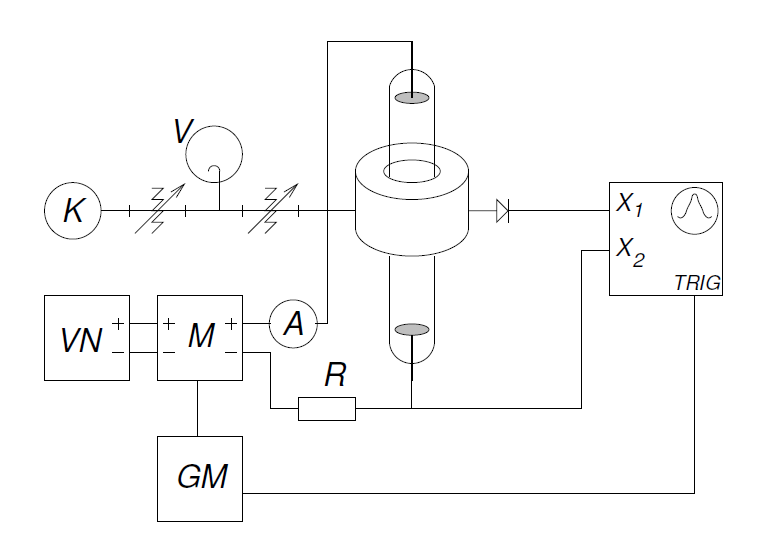
\includegraphics[width=110mm]{schema.png}
	\caption{Schéma měřící aparatury \cite{navod}.}
	\label{schema}
\end{figure}

\begin{figure}[h]
	\centering
	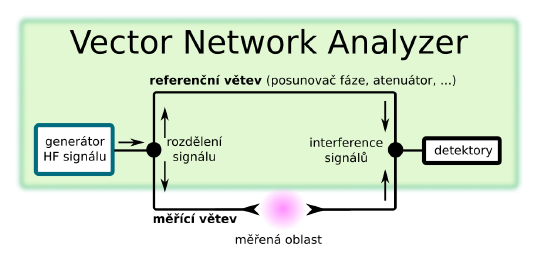
\includegraphics[width=110mm]{vna.png}
	\caption{Schéma Vector Network Analyzer (VNA) \cite{navod}.}
	\label{vna}
\end{figure}

Před měřením je potřeba VNA zkalibrovat. To se klasicky provádí pomocí definovaných
zátěží -- short, open a match. Měření probíhá následovně: Na vysokonapěťovém zdroji
měníme proud mezi hodnotami 0,2--3\,\si{\milli\ampere} a zaznamenáváme fázi a 
absolutní hodnotu parametru $S_{21}$. Odražený výkon zanedbáváme. Na VNA máme 
zapnuté 10násobné průměrování, 
čímž 
potlačíme
šum. Jelikož je zářivka už stará, mezi měřeními je potřeba s ní občas pohnout. 
Proto každé dvě měření s~určitými hodnotami proudu na zářivce vystřídáme měřením
s~nulovým proudem, tedy vypnutou zářivkou. Při zpracování dat poté vztahujeme jednotlivá
měření k~nejbližšímu s~nulovým proudem. Tímto způsobem tedy zkoumáme vliv výboje v~zářivce umístěné ve vlnovodu na procházející signál vlnovodem.

Ve výpočtech vystupuje veličina $\Delta z$, kterou jsme obecně označili jako 
úsek dráhy.
V~našem případě se jedná o~tloušťku plazmatu, kterou je potřeba odhadnout. To provedeme
pomocí geometrické úvahy ze znalosti příčného rozměru vlnovodu $a = 
86$\,\si{\milli\meter},
průměru zářivky $d$~=~$18$\,\si{\milli\meter}, délky zářivky $l = a/\sin\alpha$ 
a úhlu mezi 
zářivkou a vlnovodem 
$\alpha = 35^{\circ}$. Za
předpokladu, že zářivka má objem válce $V_v$, který následně nahradíme 
pravidelným
čtyř\-bo\-kým hranolem s objemem $V_h = V_v =ab\Delta z$, tloušťka plazmatu 
podél 
nejdelšího rozměru vlnovodu je

\begin{equation}
	\Delta z~= \frac{\pi d^2}{4a\sin\alpha} = 5,2\,\si{\milli\meter}
	%\frac{V_v}{ab} = \frac{l \pi d^2}{4ab} = \frac{b \pi d^2}{4ab\sin\alpha} =
\end{equation}

První sadu dat měříme pro oblast frekvencí 1,5--3\,\si{\giga\hertz}. 
Vlnovod přenásí energii až od určité mezní frekvence. Průřezem vlnovodu je 
obdélník a jeho delší strana $a$ určuje mezní frekvenci $f_{\text{m}} = 
\frac{c}{2a} = 1,744\,\si{\giga\hertz}$. Horní hranici 3\,\si{\giga\hertz} jsme 
zvolili kvůli nedokonalostem vlnovodu na vyšších frekvencích. Druhou sadu dat 
jsme naměřili stejným způsobem pro menší oblast frekvencí 
2,235--2,265\,\si{\giga\hertz}.

Na obr.~\ref{S21vyp} je zobrazena 
amplituda $S_{21}$ parametru pro vypnutou výbojku. Vidíme tedy propustnost 
vlnovodu a měřená mezní frekvence téměř odpovídá vypočítané. Pro následující 
grafy je $S_{21}$ parametr měřen od frekvence 1,75\,\si{\giga\hertz}. Na 
obr.~\ref{phasetofreq} a \ref{phasetofreqzoom} jsou vyneseny fázové posuvy
v~závislosti na frekvenci pro 7 různých proudů $I$ tekoucích plazmatem a pro 
širší a užší oblast frekvencí. Pozorujeme s~rostoucím proudem vyšší fázový 
posuv. Z~něj jsme dále vypočítali koncentraci elektronů v~plazmatu dle vztahu 
\eqref{eq:koncentrace} a její závislost na proudu vynesli do 
obr.~\ref{koncnai}. Pro proudy $I$~=~$0,4$--$3$\,\si{\milli\ampere} se 
koncentrace 
pohybuje řádově $n_e \approx 10^{15}$--$10^{16}$\,\si{\cubic\per\meter}. 
Typické 
hodnoty pro doutnavý výboj
$n_{e,\text{typ}}$~$\approx$~$10^{15}$--$10^{17}$\,\si{\cubic\per\meter} dle
\cite{conc} odpovídají námi naměřenými. Z~koncentrace jsme následně dle vztahu 
\eqref{eq:vd} vypočítali driftovou rychlost elektronů. Její závislost na proudu 
jsme vynesli do obr.~\ref{vd}. Závislost zde žádnou nepozorujeme, řádově se 
pohybuje $v_d \approx 10^3$\,\si{\meter\per\second}. Typickou hodnotu 
$v_{d,\text{typ}} \approx 10^4$\,\si{\meter\per\second} jsme vypočítali 
v~databázi \cite{lxcat} pro intenzitu elektrického pole $E = 
10$\,\si{\volt\per\centi\meter} a tlak $p = 100$\,\si{\pascal}.
%Zářivka už byla na konci své životnosti a nedokázali 
%jsme v~ní udržet stabilně výboj při vyšším proudu $I$, na kterém koncentrace 
%závisí. 


\begin{figure}[h]
	\centering
	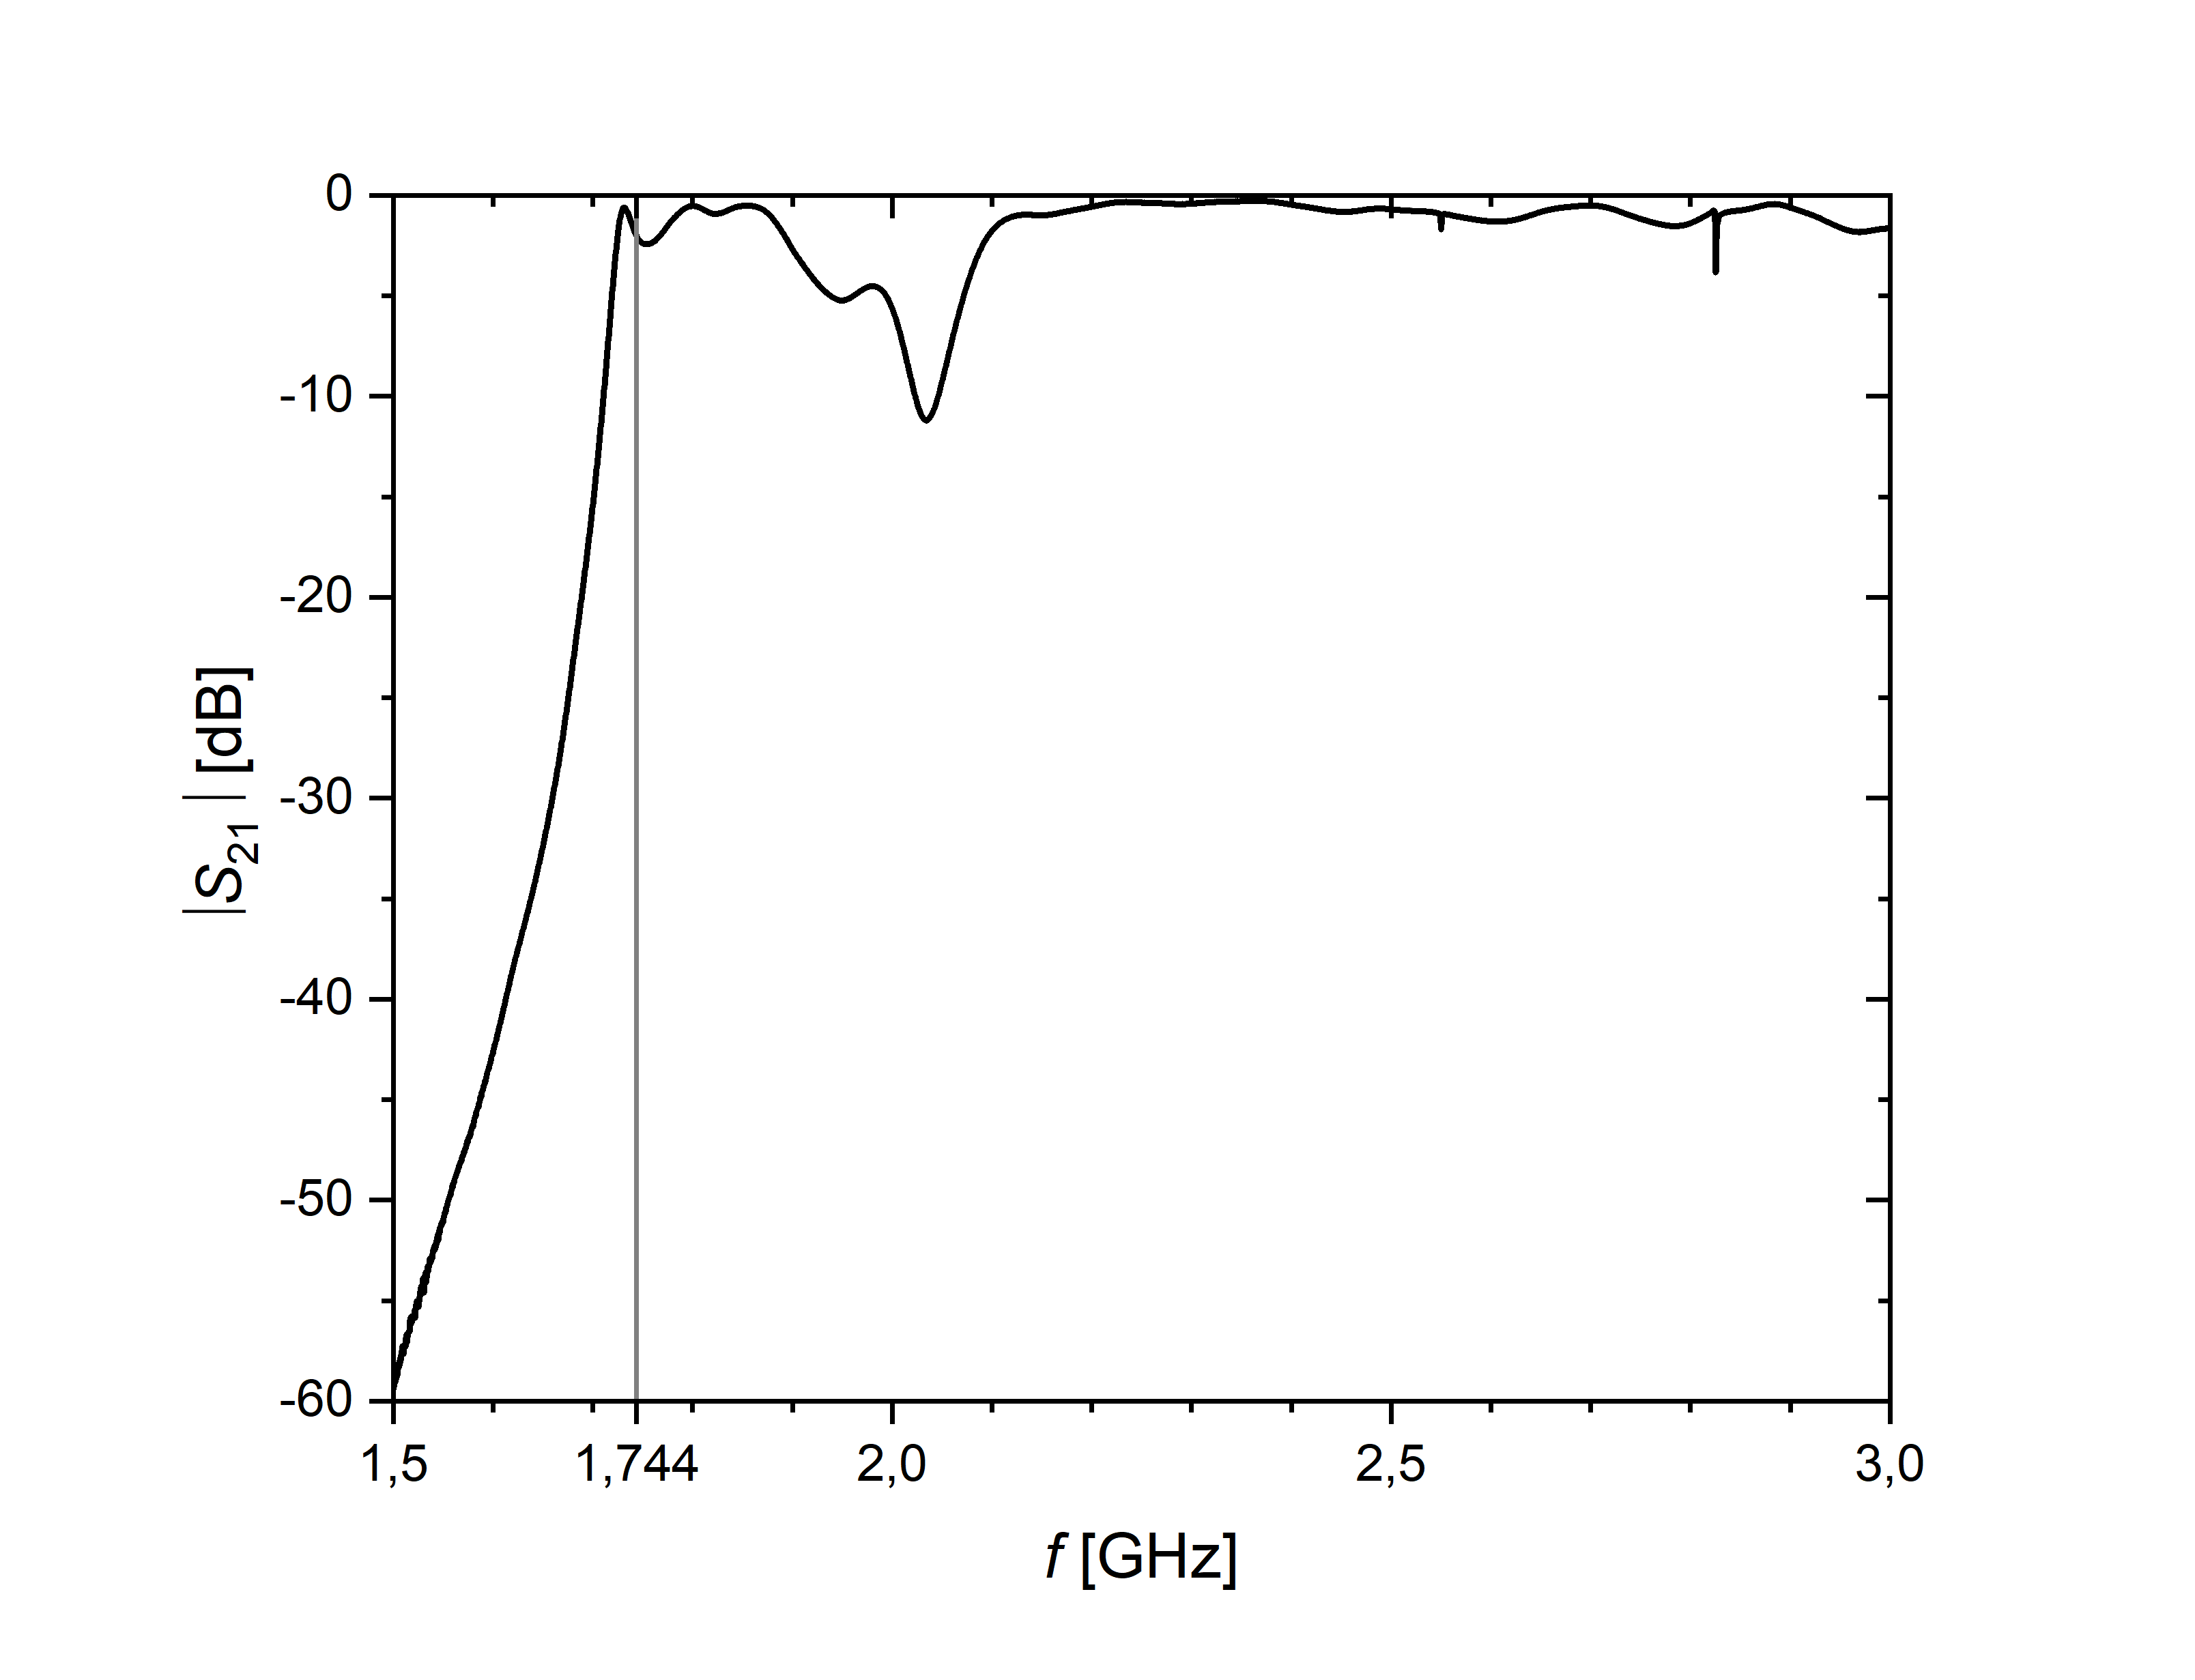
\includegraphics[width=0.9\linewidth]{S21vyp.png}
	\caption{Závislost amplitudy parametru $S_{21}$ na frekvenci se znázorněnou 
	teoretickou mezní frekvencí.}
	\label{S21vyp}
\end{figure}

\begin{figure}[h]
	\centering
	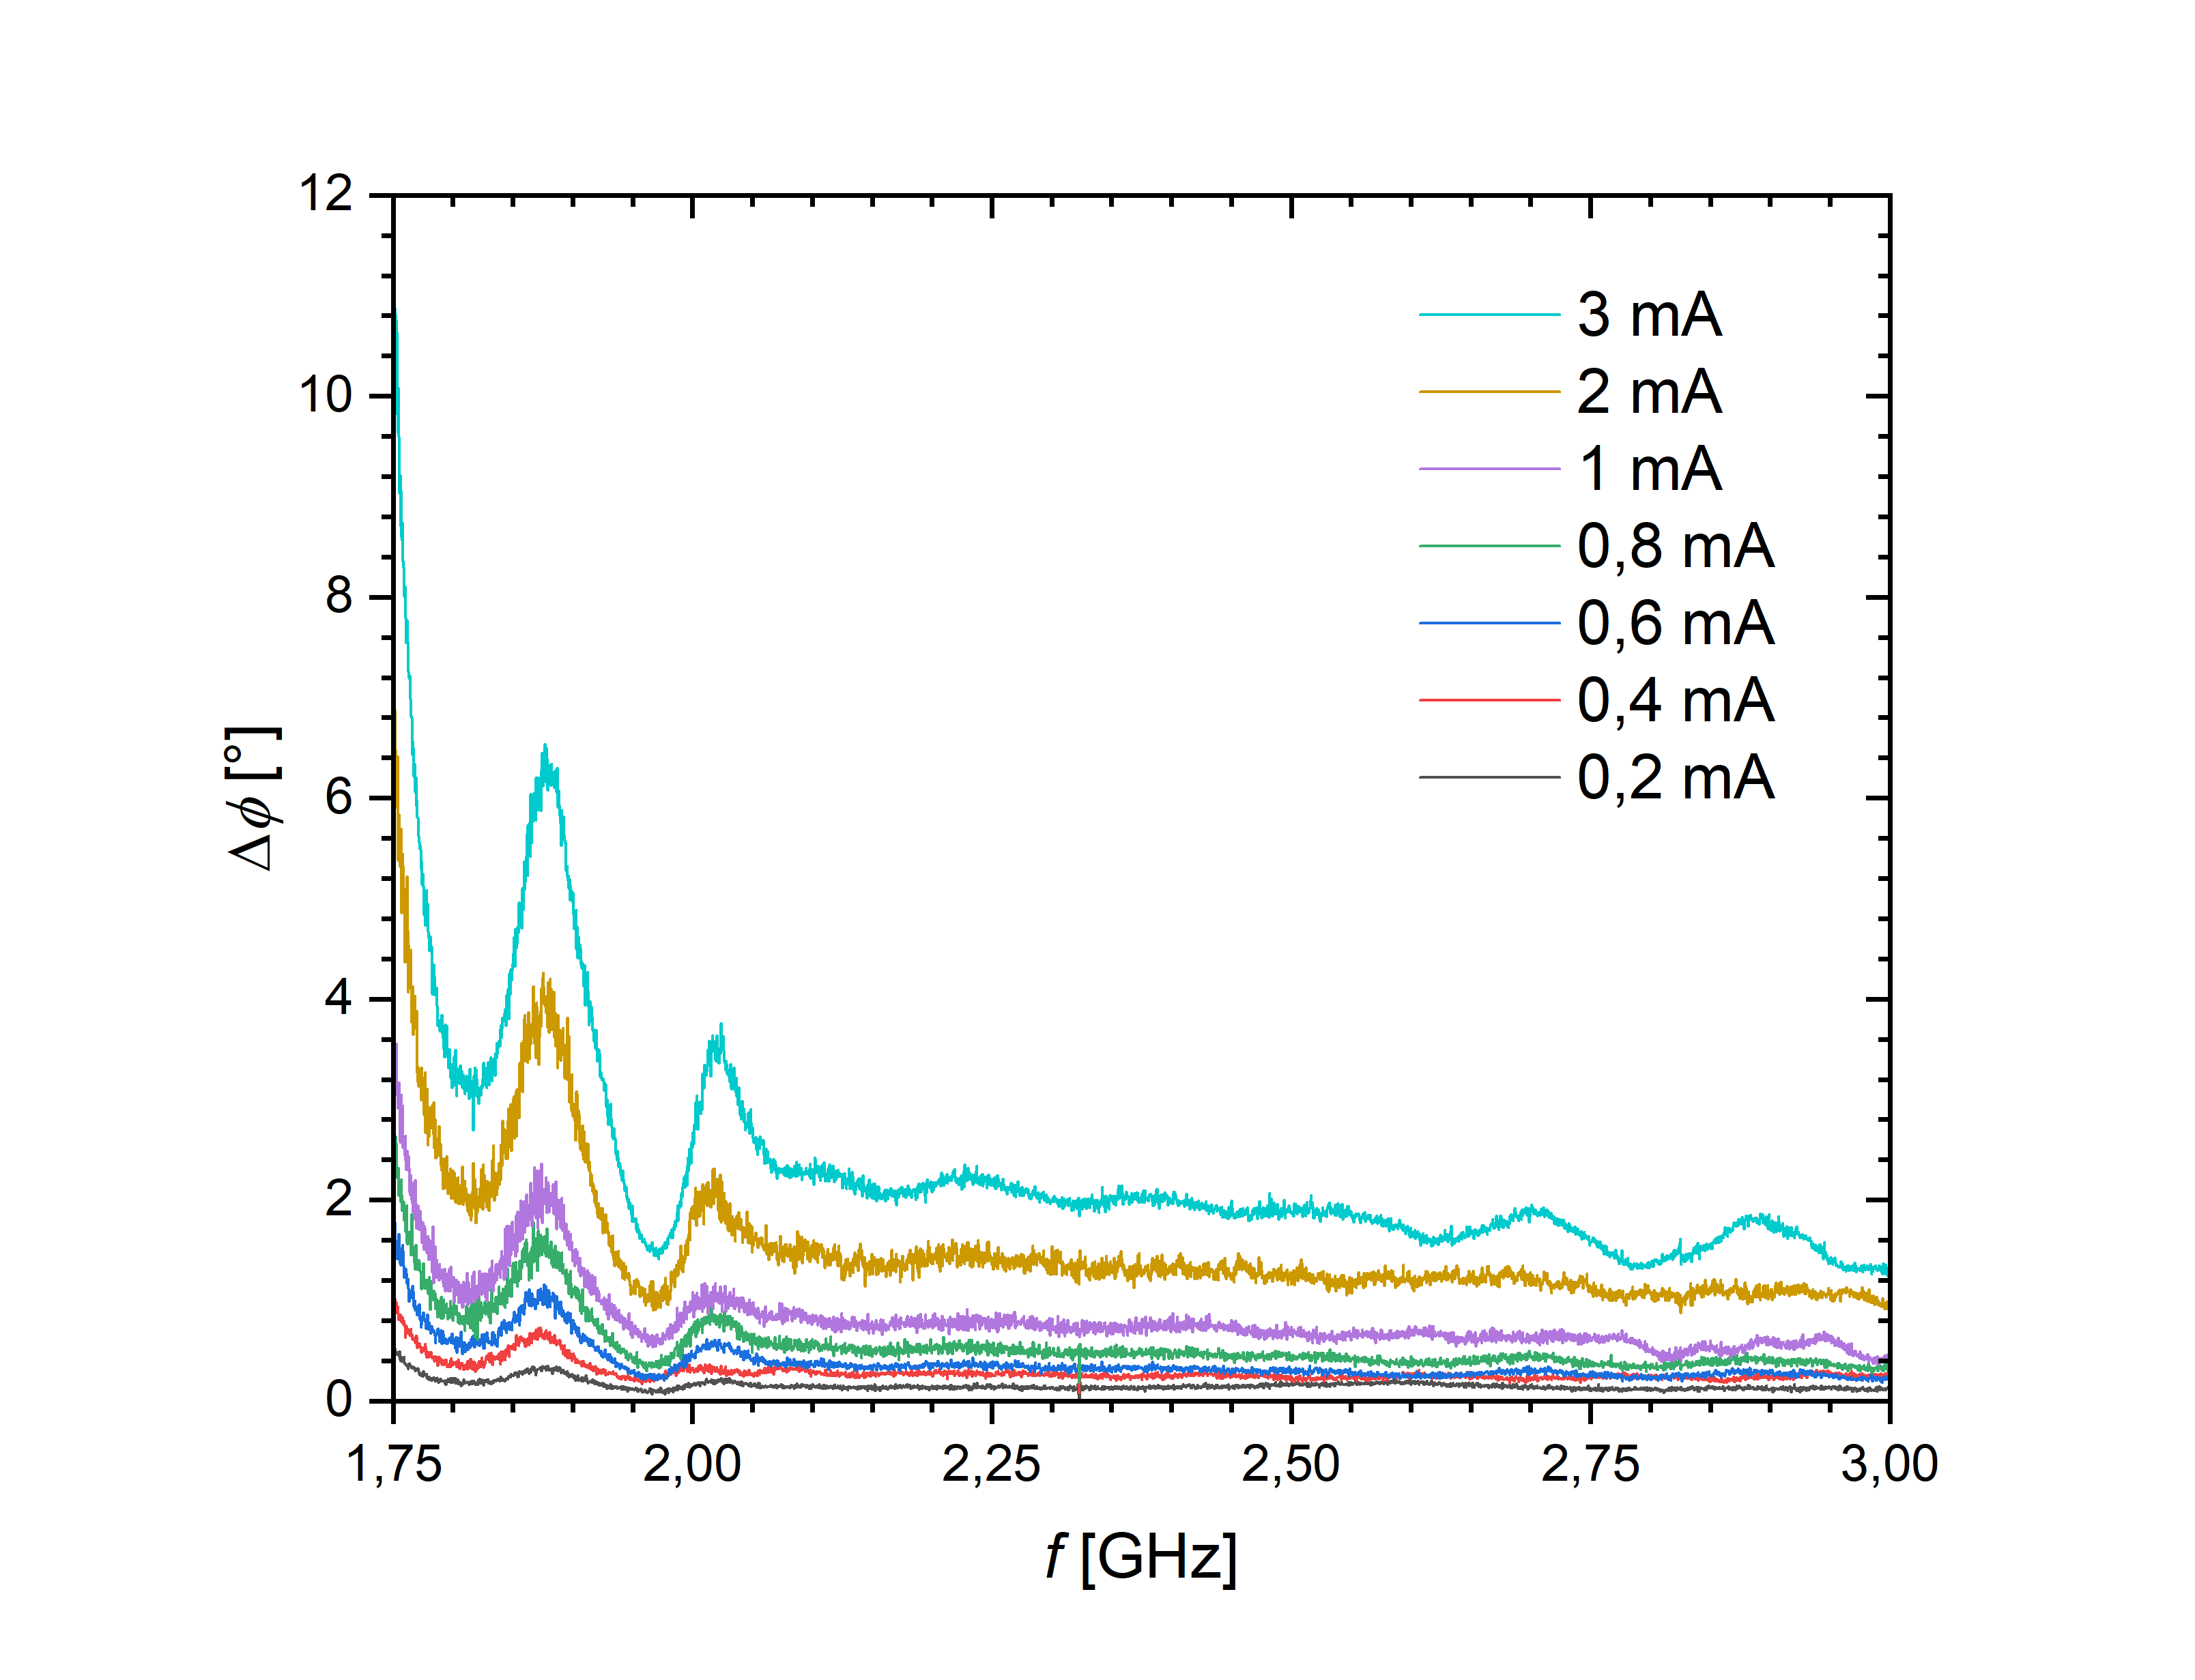
\includegraphics[width=0.9\linewidth]{phasetofreq.png}
	\caption{Závislost fázového posuvu parametru $S_{21}$ na frekvenci pro 
	širší oblast frekvencí.}
	\label{phasetofreq}
\end{figure}

\begin{figure}[h]
	\centering
	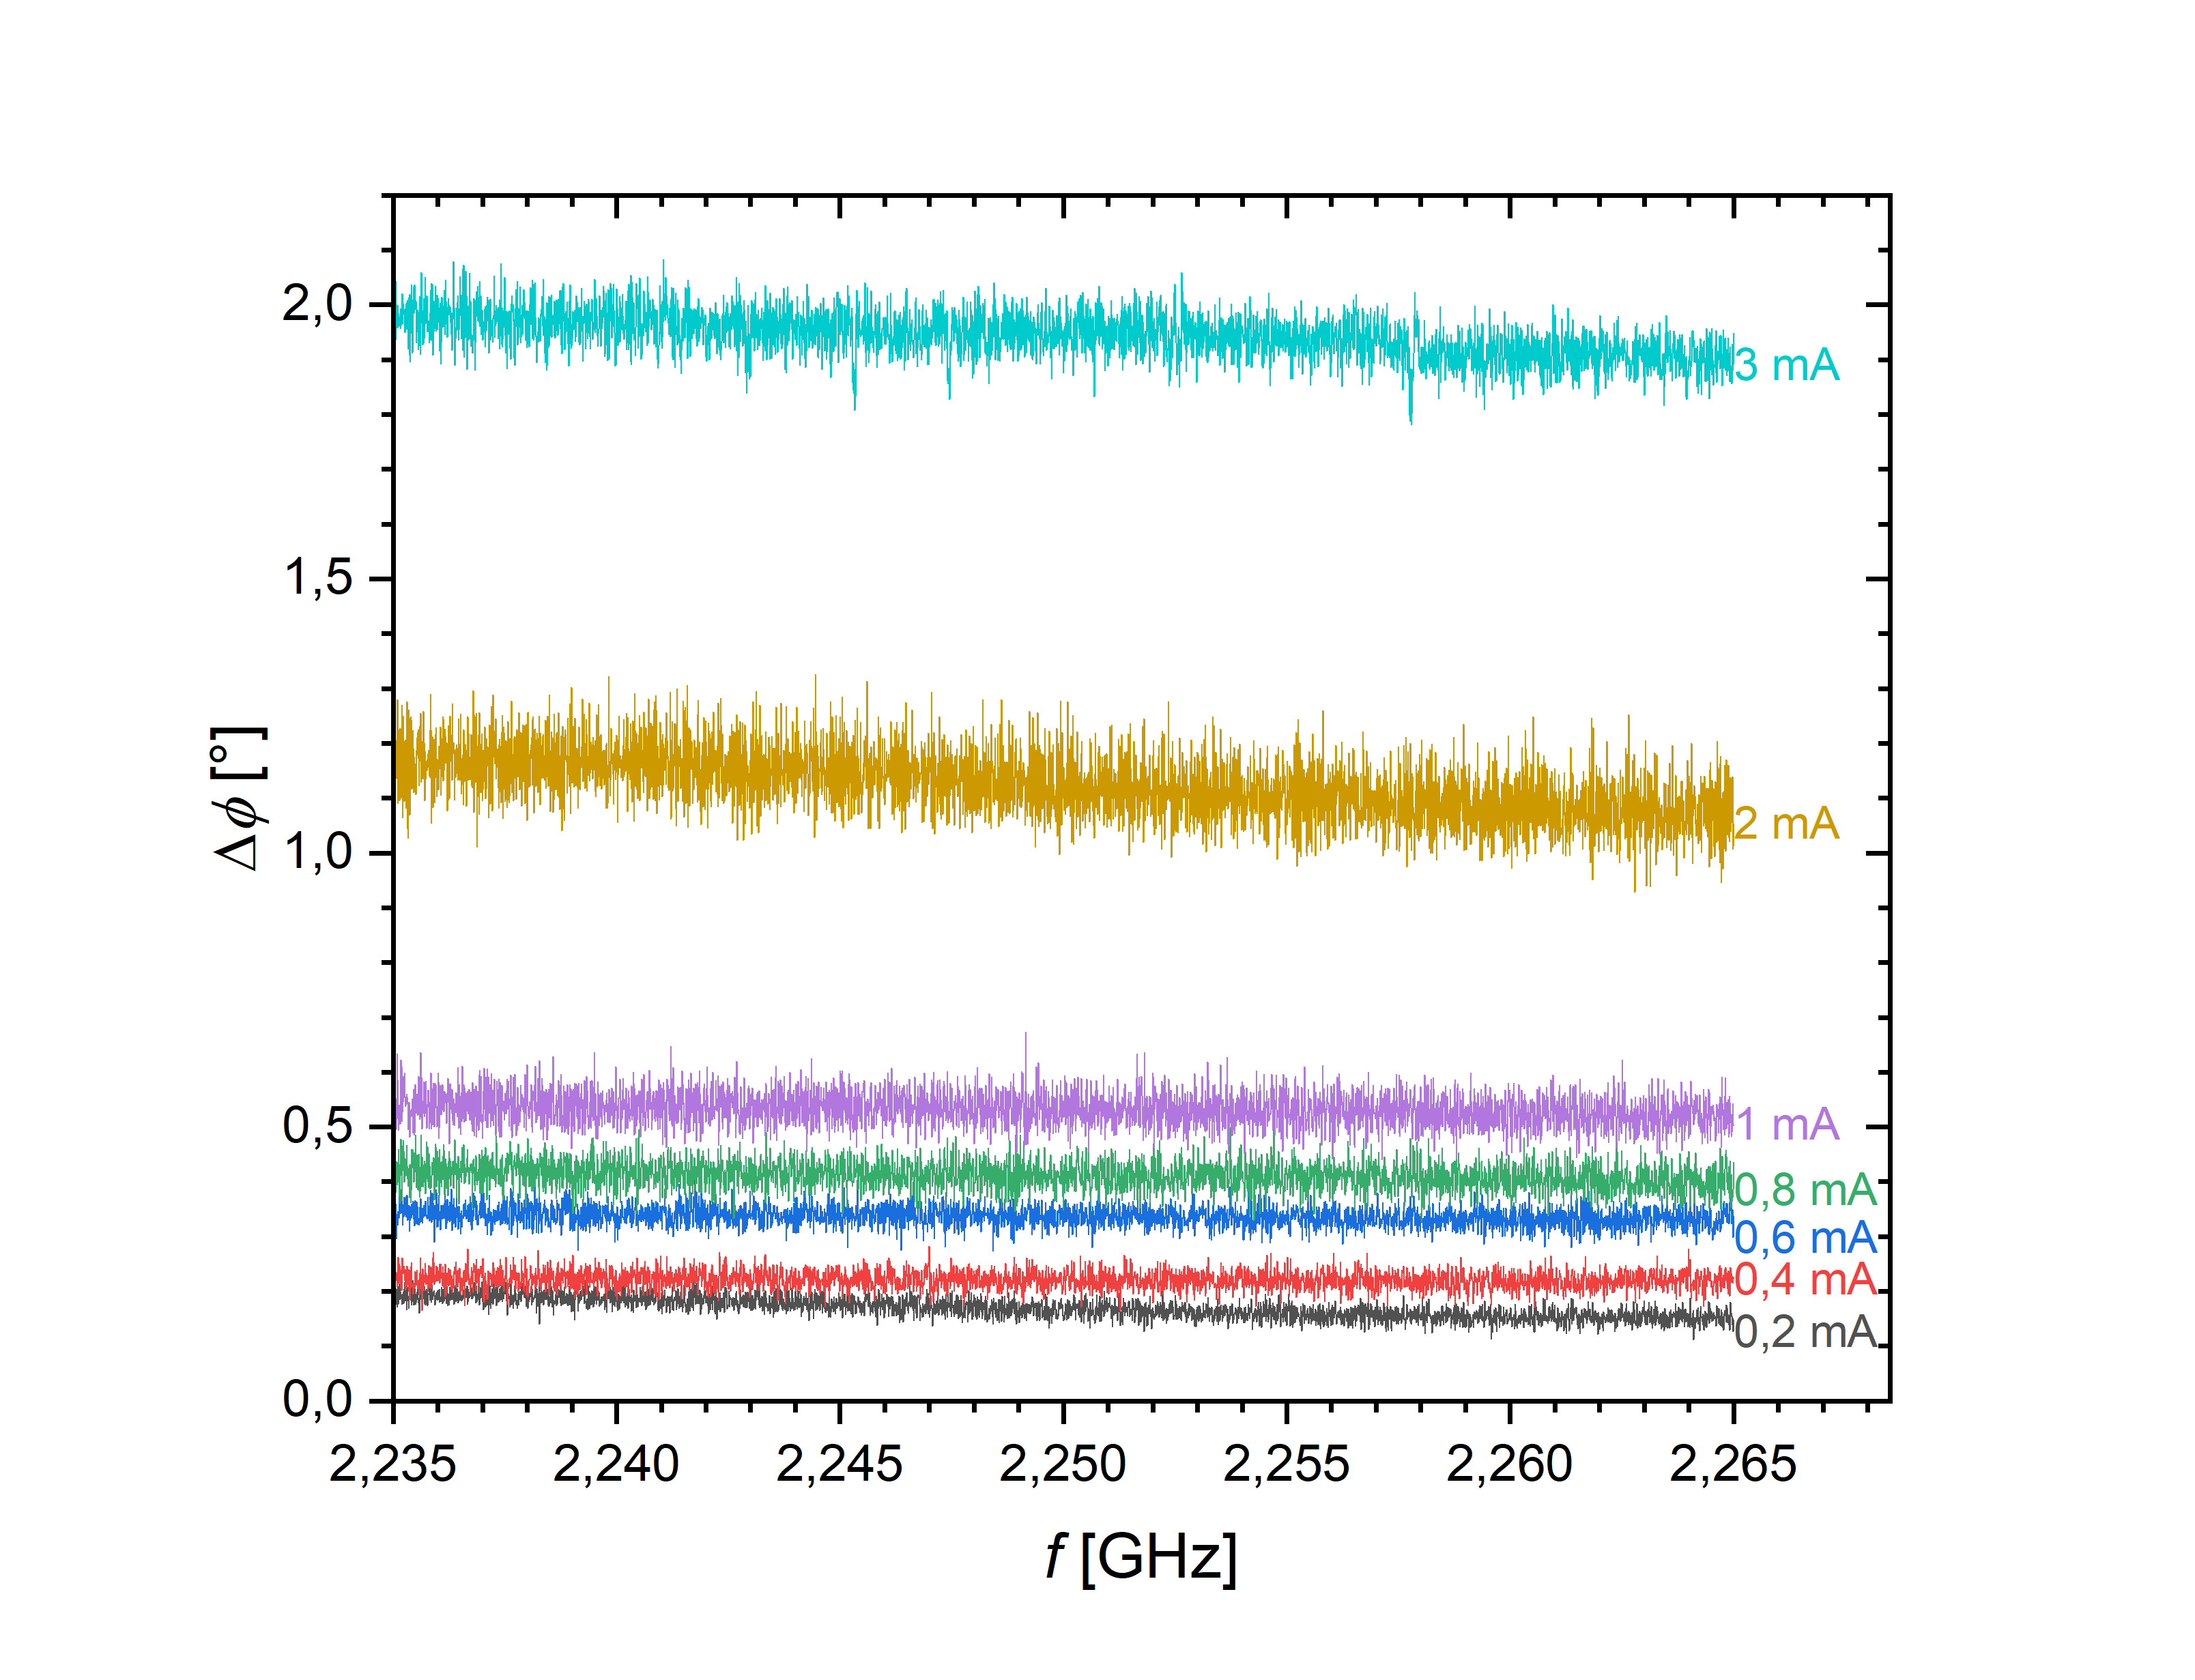
\includegraphics[width=0.9\linewidth]{phasetofreqzoom.png}
	\caption{Závislost fázového posuvu parametru $S_{21}$ na frekvenci pro 
		užší oblast frekvencí.}
	\label{phasetofreqzoom}
\end{figure}

\begin{figure}[h]
	\centering
	\includegraphics[width=0.9\linewidth]{koncnai.png}
	\caption{Závislost koncentrace elektronů na proudu pro širší a užší rozsah 
	frekvencí.}
	\label{koncnai}
\end{figure}

\begin{figure}[h]
	\centering
	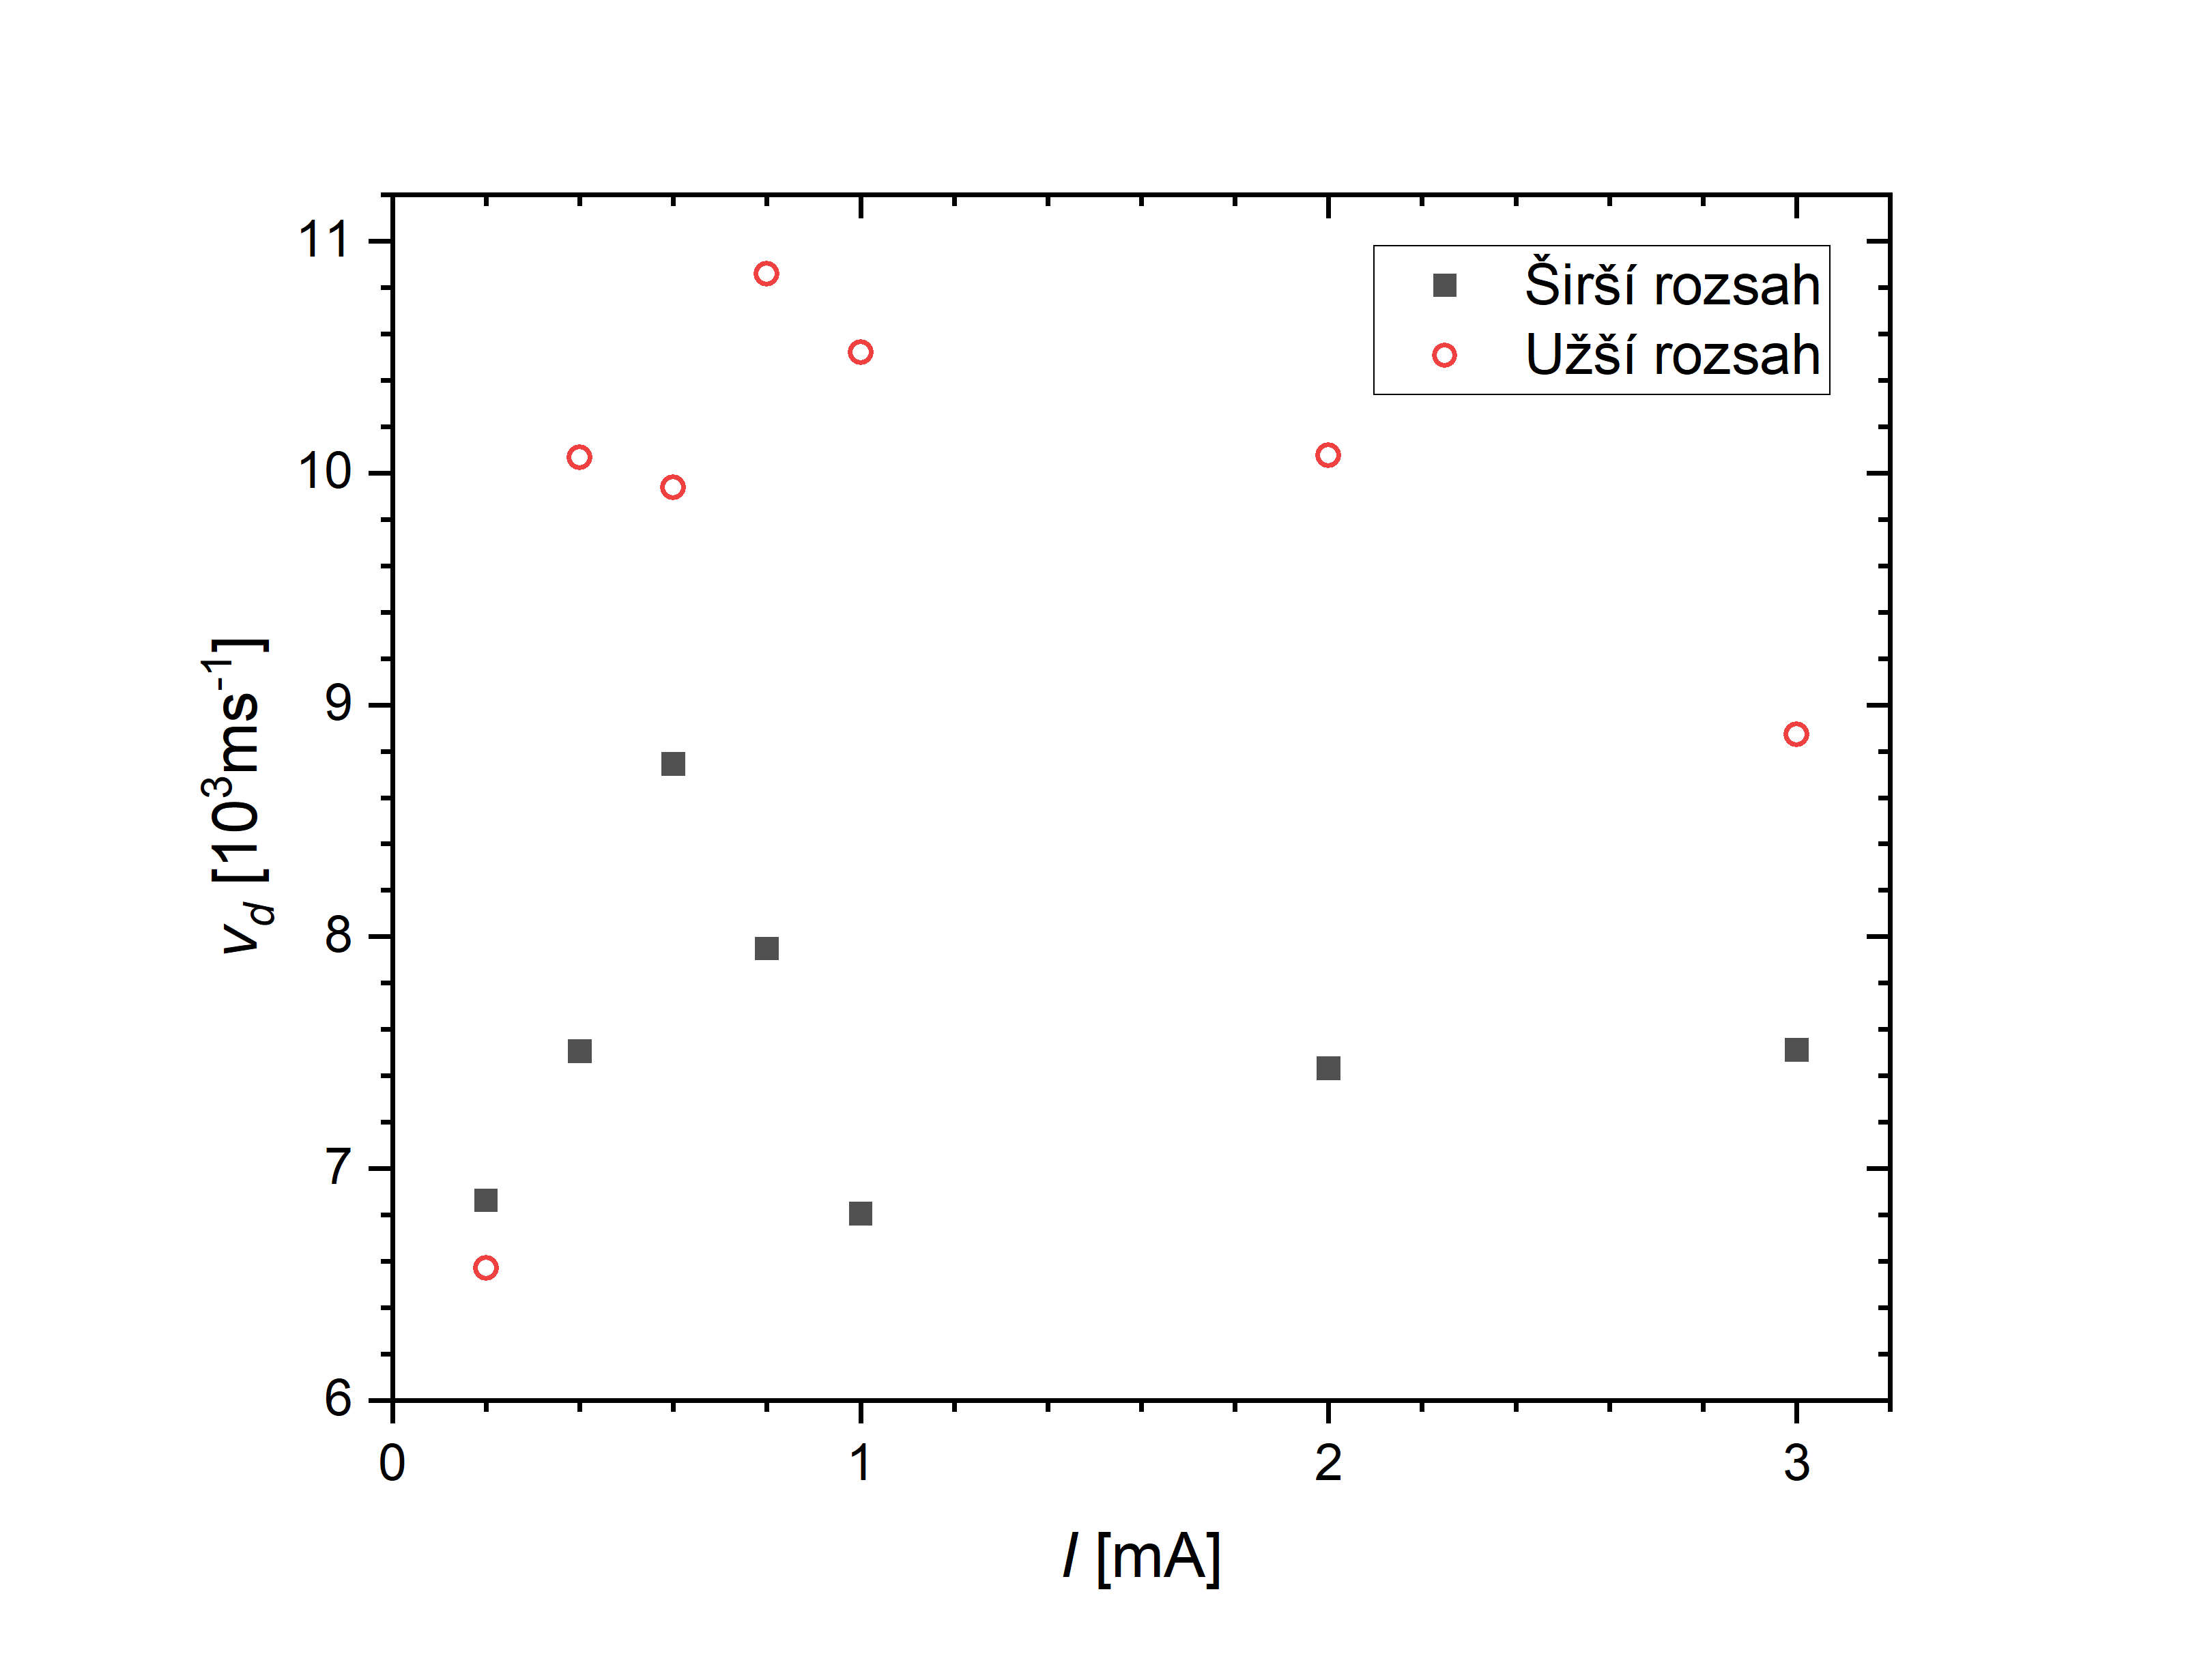
\includegraphics[width=0.9\linewidth]{vd.png}
	\caption{Závislost driftové rychlosti na proudu pro širší a užší rozsah 
		frekvencí.}
	\label{vd}
\end{figure}

\clearpage
\section{Závěr}
\par Mikrovlnnou inteferometrií jsme měřili vlastnosti běžné zářivky. Pomocí 
VNA jsme na\-mě\-ři\-li $S_{21}$ parametr, který je závislý na interakci 
elektromagnetického záření s~plazmatem. Z~něj jsme následně určili posuv 
fáze v~závislosti na frekvenci a koncentraci elektronů uvnitř zářivky. Ta 
vyšla pro proudy $I$~=~$0,4-3$\,\si{\milli\ampere} řádově $n_e \approx 
10^{15}-10^{16}$\,\si{\cubic\per\meter}. Typické 
hodnoty $n_{e,\text{typ}}$~$\approx$~$10^{15}-10^{17}$\,\si{\cubic\per\meter} 
dle 
\cite{conc} odpovídají měření. Driftová rychlost elektronů vyšla 
$v_{d}$~$\approx$~$10^3$\,\si{\meter\per\second}, přičemž typická hodnota 
$v_{d,\text{typ}} \approx 
10^4$\,\si{\meter\per\second} určena z~\cite{lxcat} je o řád vyšší.
%Nižší naměřené hodnoty jsou způsobeny limitem v proudu, který jsme byli 
%schopní přivést na zářivku a zároveň udržet stabilní výboj. Důvodem byla 
%nevyhovující zářivka na konci životnosti.

\begin{thebibliography}{10}
	\bibitem{navod} 
	Návod k praktiku: \textit{Mikrovlnná interferometrie plazmatu.} 
	Experimentální metody 2.
	\bibitem{conc}
	FRANZ, Gerhard. \textit{Low Pressure Plasmas and Microstructuring 
	Technology} 
	[online]. Berlin, Heidelberg: Springer Berlin Heidelberg, 2009 [cit. 
	2022-06-26]. ISBN 978-3-540-85848-5. Dostupné z: 
	doi:10.1007/978-3-540-85849-2
	\bibitem{lxcat}
	E. Carbone, W. Graef, G. Hagelaar, D. Boer, M.M. Hopkins, J.C. Stephens, 
	B.T. Yee, S. Pancheshnyi, J. van Dijk, L. Pitchford. \textit{Data Needs for 
	Modeling Low-Temperature Non-Equilibrium Plasmas: The LXCat Project, 
	History, Perspectives and a Tutorial.} Atoms (2021) 9 (1), 16.
\end{thebibliography}
\end{document}